\documentclass[12pt]{article}
\usepackage{graphicx}
\usepackage {color}
\usepackage{pdfpages}
\usepackage{float}
\usepackage{changebar}
\usepackage{enumitem,amssymb}
\renewcommand{\familydefault}{\sfdefault}
\usepackage[margin=1.2in]{geometry}
\usepackage{graphicx}
\usepackage{wrapfig}
\usepackage[super]{cite}
\usepackage{subcaption}
\usepackage[table]{xcolor}
\usepackage{amsmath}
\usepackage[sort, numbers]{natbib}

%%%%%%%%%%%%Defining the margins %%%%%%%%%%%%%%%%%%%%%
\textheight 9.in
\textwidth 6.5in
\topmargin -.5in
\oddsidemargin 0in
\setlength{\parskip}{\smallskipamount}

%%%%%%%%%%%%%%Specific Commands %%%%%%%%%%%%%%%%%%
\newcommand{\eg}{{\em e.g.,}}
\newcommand{\ie}{{\em i.e.,}}
\newcommand{\etc}{{\em etc.,}}
\newcommand{\etal}{{\em et al.}}
\newcommand{\degrees}{{$^{\circ}$}}
\newcommand{\micro}{{$\mu$}}


%%%%%%%%%%%%%%%%%%%%%%%%%%%% Setting to control figure placement
% These determine the rules used to place floating objects like figures 
% They are only guides, but read the manual to see the effect of each.
\renewcommand{\topfraction}{.9}
\renewcommand{\bottomfraction}{.9}
\renewcommand{\textfraction}{.1}
\renewcommand{\familydefault}{\sfdefault} %setting the san serif font

%%%%%%%%%%%%%%%%%%%%%%%% Line spacing
% Use the following command for ``double'' spacing
%\setlength{\baselineskip}{1.2\baselineskip}
% and this one for an acceptable NIH spacing of 6lpi based on 11pt
%\setlength{\baselineskip}{.9\baselineskip}
% The baselineskip does not appear to work when we include a maketitle
% command in the main file.  Something there must set the line spacing
% If we use this next command, then things seem to work.
\renewcommand{\baselinestretch}{.9}

\setcounter{secnumdepth}{0} %make no numbers but have a table of contents


\begin{document}

\title{Lab 4, Neuron and Backyard Brains}
\author{Jake Bergquist, u6010393}
\maketitle
\tableofcontents
\newpage

\section{Introduction}
In biology the study of structure and function relationships relies in part on various imaging techniques in order to assess the physical structure and layout of biological materials. At an organ and even to some extend a tissue level methods such as visible light microscopy cna be beneficial for resolving anatomical and cellular structure. However, when it comes to assessing biological specimens at a cellular and sub cellular level, higher resolution and finer detail are often required. Many of these methods of imaging of cellular level structures and organization rely on fluorescent labeling. This is a method by which specific substructures of a cell are tagged with material can be identified using florescent microscopy. The materials used to tag the cells are typically proteins conjugated to florescent molecules (in many cases a primary antibody protein attaches to the structure of interest and secondary antibody attaches to the primary antibody and carries the fluorescent molecule) or in some cases the fluorescent molecules themselves can act as specific or general tags. The targets of these tags range from specific proteins, protein subdomains, amino acid sequences, DNA, and other cellular components. Tissue samples are fixed and tagged using these various systems with several different fluorescent tags used simultaneously to assess multiple structures of interest within one tissue and there localization relative to one another. These fluorescent tags are visualized using fluorescent microscopy. This is a process by which the fluorescent molecules are induced to emit a wavelength of light which is specific to each fluorescent molecule. Each fluorescent molecule is characterized by an excitation and emission spectrum, which describes the wavelengths of light that will excite the electrons of the florescent molecule (the excitation spectrum), and what wavelength of light is released when the electrons fall back to their basal energy state (the emission spectrum). By shining light onto the specimen int he excitation spectrum and recording light from the emission spectrum the specific fluorescent molecules can be imaged. By adjusting the focus of the light shined onto and collected from the specimen down to a single point and scanning this point across the specimen and through its depth the 2D and 3D structure of the specimen can be resolved.

The specific tissue of interest in this report was taken from human atria. These tissue samples were labeled with wheat  germ  agglutinin (WGA)  conjugated  to  AlexaFluor-488 which stains the extracellular space and a stain for connexin43 (Cx43) with AlexaFluor-594. This allowed us to separately resolve the extracellular space which defines the spae of the cardiac myocytes as well as the spatial arrangement of the gap junctions (which contain two hexamers of connexin43/other connexins). Cardiac myocytes are typically cylindrical or ``brick" shaped cells that arrange into filaments and sheets.\cite{Woodcock2005} The gap junctions composed of two hexamers of connexins form open channels between cardiac myocytes. Gap junctions are found across the cell membrane where the myocytes is connected with its neighbor but the concentration is higher at the terminal ends of the myocytes.\cite{Mese2007} These gap junctions allow for free passage of ions and small molecules from cell to cell. This allows for the electrical activity of one cell such as the initiation of an action potential, to propagate to the neighboring cells. In this way the activating wavefront of cardiac electrical activity propagates from cell to cell in the heart. This leads to a synchronized and ordered wave of electrical activation across the heart which in turn leads to an ordered contraction of the heart.\cite{Mese2007} The arrangement of gap junctions throughout the cell plays a critical role in controlling the direction and propagation properties of this excitation wave. As such, visualizing the structure and arrangement of gap junctions in myocytes can be informative when examining disease states where gap junction remodeling is implicated.

\section{Methods}
\subsection{Image Acquisition}
Atrial tissue samples were obtained fromt he lab instructor. These samples had be prepared with WGA conjugated to AlexaFluor-488 stain and an anti-connexin43 antibody conjugated to AlexxaFluor-594. The sample was imaged using excitation spectra of 488 nm (for the WGA 488 fluorophore) and 594 nm (for the connexin 594 fluorophore). Recording were done with either the hybrid photomultiplier or the conventional photomultiplier. The effect of increasing laser power, changing photomultiplier gain, and changing pinhole size were examined. Additionally a 3D stack of images was acquired by sampling at 50 depths through the tissue.
\par{Baseline:} A baseline image was acquired with a pinhole size of 1 AU, 1024 x 1024 pixels (288x288 nm pixel size), and laser power of 3 and 2 for the 488 nm and 594 nm lasers respectively. The hybrid photomultiplier was used with default settings. Imaging was done for the WGA emission spectra for all image parameter sets and at the connexin 43 emission spectra for the baseline parameter set.
\par{Laser Power:} A 2D image was taken with increased laser power. The 488 nm laser power was increased from 3 to 6, and the 594 nm laser was increased from 2 to 4. All other parameters followed baseline parameters.
\par{Gain Adjustment:} A 2D image was acquired using the conventional photomultipliers with a gain of 500 V and 700 V. All other parameters followed the baseline parameters.
\par{Pinhole Size:} A 2D image was acquired with a pinhole size of 3 AU. All other parameters followed the baseline parameters.
\par{3D Stack: } A 3D stack was acquired at a resolution of 512 x 512 pixels per stack ( 758 x 758 nm pixel size). A total of 50 slices were taken making for a 512 x 512 x 50 image stack for both fluorophore channels. All other parameters followed the baseline parameters.

\subsection{Image Processing}
Fir each of the 2d images the .liff stack was imported to the FIJI processing system. Each image was manually adjusted for brightness and contrast to provide the clear visualization. Due to the requirements of the lab, each image was set at a constant relative scaling from 0 to 64\% of the intensity histogram when the brightness and constrast was adjusted. For each 2d image the histogram of signal intensities was assessed for the WGA channel. A threshold was applied at an intensity value of the mode plus one standard deviation. This threshold was used to make a selection in the image of the background signal. The histogram of this background was assessed to calculate the standard deviation of the background. The selection was then inverted to attain a selection of the signal. The histogram of the signal was used toc alculate the mean signal intensity, which when divided by the background standard deviation produced the signal to noise ratio (SNR) of the image. The WGA channel was visualized along with the total signal histogram for each parameter manipulation. Additionally the baseline image cas was visulized using a merged image of the WGA and CX43 channels, with the WGA chanel colored red and the cx43 channel colored green.


\section{Results}
The WGA and connexin signals using baseline parameters are shown with their accompanying histograms of pixel intensity in Figure~\ref{fig:wga_base} and Figure~\ref{fig:cx43_base} respectively. These images are combined in Figure~\ref{fig:base_merge}. Finally a binary image was produced from the WGA baseline image by thresholding at mode plus one standard deviation(Figure~\ref{fig:base_binary}). This image was annotated to highlight a single myocyte and some of the t-tubule invaginations. Using the count function the number of signal pixels (322,524) and background pixels (727,052) were calculated in order to compute the fraction of extracellular space. The signal represents the extracellular space stained by WGA and the background is the intracellular space, thus the fraction of extracellular space is (extracellular / (intracellular + extracellular)) 0.22.

\begin{figure}[H]
	\begin{subfigure}{.5\textwidth}
		\centering
		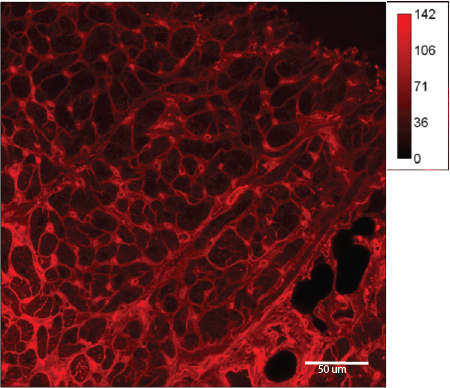
\includegraphics[width=.95\linewidth]{FinalFigures/WGA_Baseline.png}
		\caption{}
		\label{fig:wga_b}
	\end{subfigure}%
	\begin{subfigure}{.5\textwidth}
		\centering
		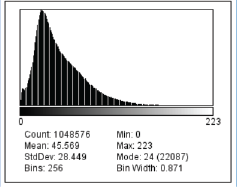
\includegraphics[width=.95\linewidth]{FinalFigures/WGA_Baseline_Hist.png}
		\caption{}
		\label{fig:wga_b_hist}
	\end{subfigure}
	\caption{Baseline WGA signal using baseline settings and the hybrid photomultiplier. The acquired signal is shown (a) in red with a 50 micron scale bar in the bottom right. The accompanying signal intensity histogram (b) shows a mode intensity of 24 with standard deviation of 28.449.}
	\label{fig:wga_base}
\end{figure}


\begin{figure}[H]
	\begin{subfigure}{.5\textwidth}
		\centering
		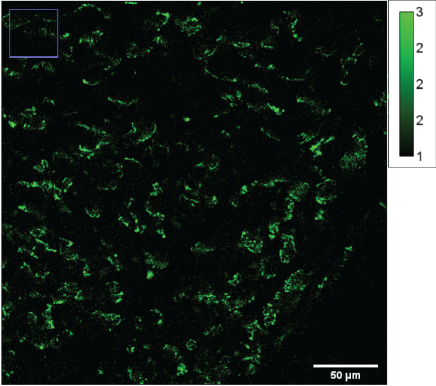
\includegraphics[width=.95\linewidth]{FinalFigures/CX43_Baseline.png}
		\caption{}
		\label{fig:cx43_b}
	\end{subfigure}%
	\begin{subfigure}{.5\textwidth}
		\centering
		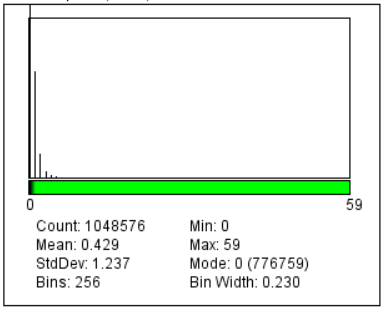
\includegraphics[width=.95\linewidth]{FinalFigures/CX43_baseline_Hist.png}
		\caption{}
		\label{fig:cx43_b_hist}
	\end{subfigure}
	\caption{Baseline connexin signal using baseline settings and the hybrid photomultiplier. The acquired signal is shown (a) in green with a 50 micron scale bar in the bottom right. The accompanying signal intensity histogram (b) shows a mode intensity of 0 with standard deviation of 1.237.}
	\label{fig:cx43_base}
\end{figure}

\begin{figure}[H]
	
		\centering
		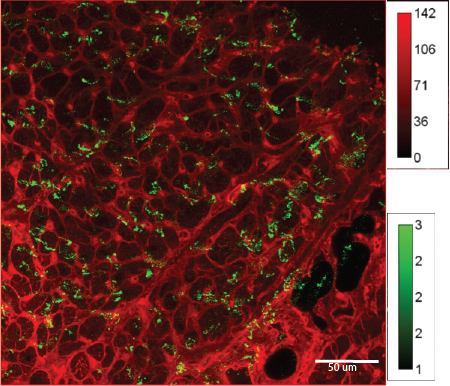
\includegraphics[width=.95\textwidth]{FinalFigures/BaselineMerge.png}
		
	\caption{Baseline connexin and WGA signal merged using baseline settings and the hybrid photomultiplier. The acquired signal is shown with connexin signal in green and WGA snal in red. A 50 micron scale bar is shown in the bottom right.}
	\label{fig:base_merge}
\end{figure}

\begin{figure}[H]
	
	\centering
	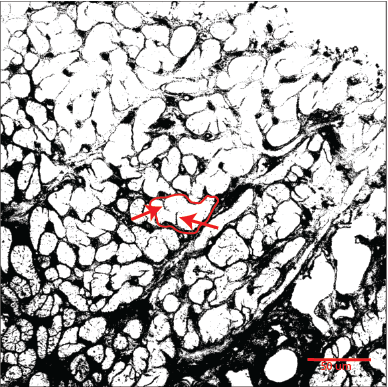
\includegraphics[width=.95\textwidth]{FinalFigures/WGA_Baseline_Binary.png}
	
	\caption{Binary image of baseline WGA signal after applying a threshold of mode + standard deviation. A 50 micron scale bar is shown in the bottom right. One myocyte is outlined in red with arrows pointing to invaginations of the t-tubular network.}
	\label{fig:base_binary}
\end{figure}

The next image shows a variation in the laser power. The WGA excitation laser power was increased by a factor of 2 from 3 to 6. This resulted in the image and accompanying histogram seen in Figure~\ref{fig:wga_laser}. When scaled to 64\% of total pixel intensity as the first images it is clear that the resulting image is much brighter (Figure~\ref{fig:wga_l}). The signal histogram is also much more spread with the mean closer to the center of the histogram.


\begin{figure}[H]
	\begin{subfigure}{.5\textwidth}
		\centering
		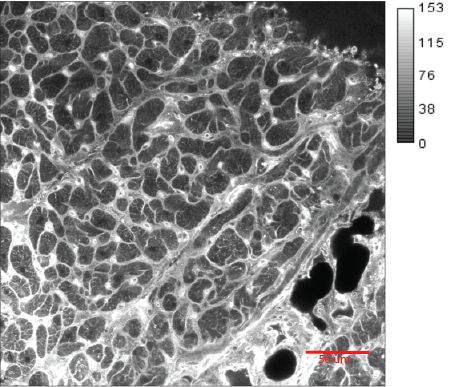
\includegraphics[width=.95\linewidth]{FinalFigures/WGA_2xlaser.png}
		\caption{}
		\label{fig:wga_l}
	\end{subfigure}%
	\begin{subfigure}{.5\textwidth}
		\centering
		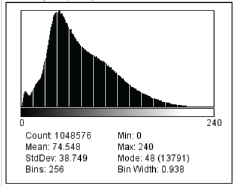
\includegraphics[width=.95\linewidth]{FinalFigures/WGA_IncreasedLaser_Hist.png}
		\caption{}
		\label{fig:wga_l_hist}
	\end{subfigure}
	\caption{WGA signal at 6 (2x) intensity. The acquired signal is shown (a) in red with a 50 micron scale bar in the bottom right. The accompanying signal intensity histogram (b) shows a mode intensity of 48 with standard deviation of 38.749.}
	\label{fig:wga_laser}
\end{figure}

The next images show the results of utilizing the conventional photomultiplier at two different gains. The 500 V gain setting is shown in Figure~\ref{fig:wga_pmt_low} which shows a much narrower histogram centered closer to the low extrema results in a lower intensity image (when scaled to 64\% of maximum pixel intensity). Increasing the gain to 700 V (Figure~\ref{fig:wga_pmt_high}) results in a more spread histogram and a brighter image.

\begin{figure}[H]
	\begin{subfigure}{.5\textwidth}
		\centering
		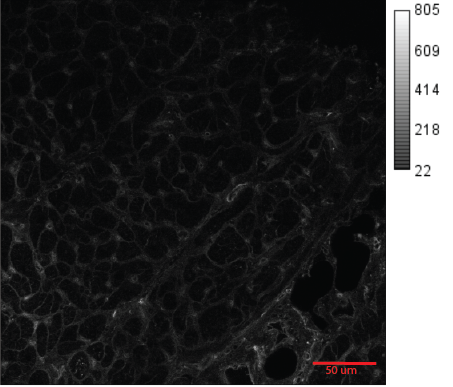
\includegraphics[width=.95\linewidth]{FinalFigures/WGA_PMT_low.png}
		\caption{}
		\label{fig:wga_pmt_l}
	\end{subfigure}%
	\begin{subfigure}{.5\textwidth}
		\centering
		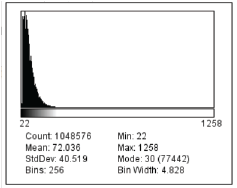
\includegraphics[width=.95\linewidth]{FinalFigures/WGA_PMT_low_hist.png}
		\caption{}
		\label{fig:wga_pmt_l_hist}
	\end{subfigure}
	\caption{WGA signal using the traditional photomultiplier tube at a gain of 500 V. The acquired signal is shown (a) in red with a 50 micron scale bar in the bottom right. The accompanying signal intensity histogram (b) shows a mode intensity of 30 with standard deviation of 40.519.}
	\label{fig:wga_pmt_low}
\end{figure}

\begin{figure}[H]
	\begin{subfigure}{.5\textwidth}
		\centering
		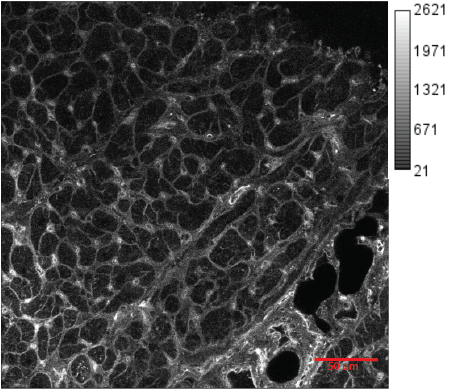
\includegraphics[width=.95\linewidth]{FinalFigures/WGA_PMT_high.png}
		\caption{}
		\label{fig:wga_pmt_h}
	\end{subfigure}%
	\begin{subfigure}{.5\textwidth}
		\centering
		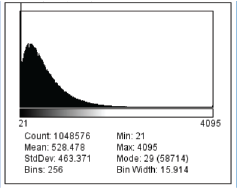
\includegraphics[width=.95\linewidth]{FinalFigures/WGA_PMT_High_Hist.png}
		\caption{}
		\label{fig:wga_pmt_h_hist}
	\end{subfigure}
	\caption{WGA signal using the traditional photomultiplier tube at a gain of 700 V. The acquired signal is shown (a) in red with a 50 micron scale bar in the bottom right. The accompanying signal intensity histogram (b) shows a mode intensity of 29 with standard deviation of 463.371.}
	\label{fig:wga_pmt_high}
\end{figure}

The final parameter of manipulation is an increase of the pinhole size to 4 AU, which results in the image seen in Figure~\ref{fig:wga_pinhole}. This image show a much wider histogram with much brighter signal.

\begin{figure}[H]
	\begin{subfigure}{.5\textwidth}
		\centering
		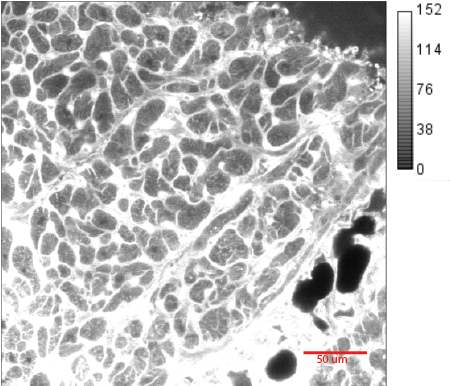
\includegraphics[width=.95\linewidth]{FinalFigures/WGA_pinhole.png}
		\caption{}
		\label{fig:wga_pin}
	\end{subfigure}%
	\begin{subfigure}{.5\textwidth}
		\centering
		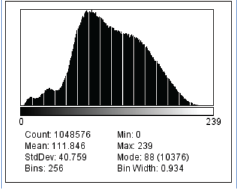
\includegraphics[width=.95\linewidth]{FinalFigures/WGA_Pinhole_Hist.png}
		\caption{}
		\label{fig:wga_pin_hist}
	\end{subfigure}
	\caption{WGA signal a pinhole of 4 A. The acquired signal is shown (a) in red with a 50 micron scale bar in the bottom right. The accompanying signal intensity histogram (b) shows a mode intensity of 88 with standard deviation of 40.759.}
	\label{fig:wga_pinhole}
\end{figure}

The z profile for the 3D stack of images is shown in Figure~\ref{fig:xy_plane}. Also depicted are two images of the xz plane, one with the same scaling of all the previous images (65\% of maximum intensity) and another with 10\% of maximum intensity as the maximum for scaling. The latter produces a more clear image. The histogram for the 3D stack is shown in Figure~\ref{fig:zhist}, showing a skewed narrow distribution. Table~\ref{tab:SNR} shows the measurements and accompanying SNRs calculated for each parameter set.

\begin{figure}[H]
	\begin{subfigure}{.95\textwidth}
		\centering
		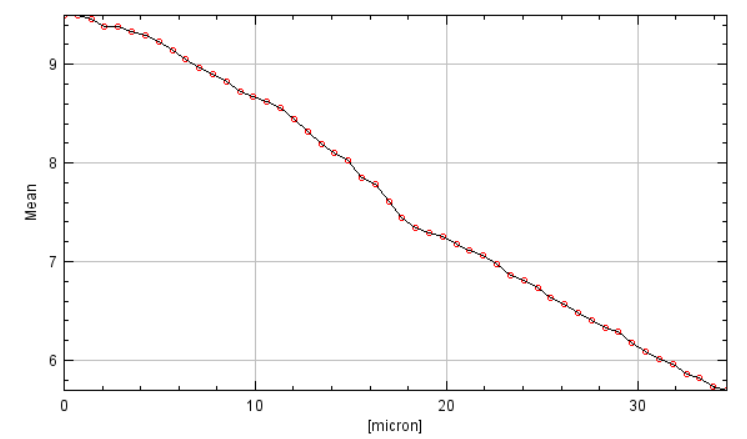
\includegraphics[width=.95\linewidth]{FinalFigures/Z_profile.png}
		\caption{}
		\label{fig:zprof}
	\end{subfigure}%
\\
	\begin{subfigure}{.95\textwidth}
		\centering
		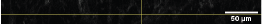
\includegraphics[width=.95\linewidth]{FinalFigures/xy_lowBright.png}
		\caption{}
		\label{fig:xy_low}
	\end{subfigure}%
\\
	\begin{subfigure}{.95\textwidth}
		\centering
		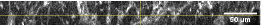
\includegraphics[width=.95\linewidth]{FinalFigures/xy_highBright.png}
		\caption{}
		\label{fig:xy_high}
	\end{subfigure}%
	\caption{WGA signal in the 3D stack. The z profile (a) is plotted through the depth of the z slices. Using the standard 64\% of maximum intensity to adjust birhgness results in a dim xy slice (b), whereas adjusting to 10\% of maximum intensity results in a clearer xy plane (c).}
	\label{fig:xy_plane}
\end{figure}

\begin{figure}[H]
	
	\centering
	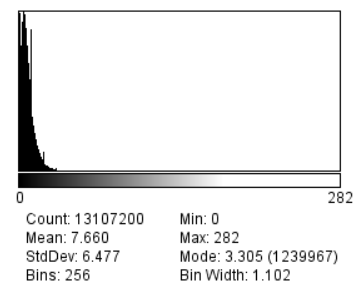
\includegraphics[width=.75\textwidth]{FinalFigures/zstackHist.png}
	
	\caption{Histogram of the full wga 3d volume.}
	\label{fig:zhist}
\end{figure}


\begin{table}[H]
	\caption{Numerical calculation of SNR for each of the parameter variations.}
	\centering
	\begin{tabular}{|r|r|r|r|} \hline
		
		Parameters&Signal Mean&Background STD&SNR\\
		\hline
		Baseline&78.59&12.12&6.44\\
		2X laser&119.39&19.27&6.20\\
		PMT 500 V&108.44&12.32&8.80\\
		PMT 700 V&930.71&137.79&6.75\\
		4 A pinhole&156.80&25.88&6.06\\
		\hline
	\end{tabular}
	\label{tab:SNR}
\end{table}




\section{Discussion}

The 4 parameter manipulations from the baseline parameter set were the increasing of laser power by a factor of 2, using a conventional Photomultiplier at 500 V and 700 V, and increasing the pinhole size from 1 AU to 4 AU. Increasing the laser power results in a slight decrease in SNR along with a shift in the histogram to the right and a brighter image. The change in SNR is marginal, however it could be caused by some saturation of the signal leading to the observed lower SNR. The structures in the image (Figure~\ref{fig:wga_l}) appear more clear and easier to distinguish. It is important to avoid saturation in the imaging process as this can cause a loss of resolution of those structures which become saturated. An additional source of noise in the 2X laser results could be due to increased laser noise at higher power, although this is though to be negligible.

Switching from a hybrid to a conventional photomultiplier has several trade-offs. Conventional photomultipliers are typically noisier and require high voltage, but are less expensive and measure current with adjustable gain dictated by the voltage supplied. Hybrid models are based on a combination of technologies and measure voltage current pulses. The conventional photomultipliers in this case also produced maximum signal intensity values an order of magnitude or two higher than the hybrid version. The absolute values of pixel intensity cannot be compared across images for multiple reasons. Between imaging sessions there are some amounts of photo-bleaching whereby the fluorescent compounds degrade at a certain when excited according to the strength of the excitation light, resulting in variable intensities from image to image. Additionally the process of capturing an image using photomultipliers is a semi stochastic process based on the physical principles of the amplification of electrons cascading through the photomultiplier. There are several sources of noise in the acquisition of the flourescent images, such as the variability in the excitation and emission of the fluorophores, the excitation light itself, the photomultiplier, and power noise. For these reasons the images can only be compared based on relative intensity values, not absolute. The conventional photomultiplier surprisingly produced a SNR that was higher than the hybrid at both gain levels (Table~\ref{tab:SNR}). However this could be explained by the method by which signal and noise were identified. As perscribed by this lab proceedure, signal was isolated from noise by a threshold of mode+std of the entire signal. Visual inspection of this threshold showed that the signal portion clearly included patchy and grainy noise, thereby skewing the calculation. Additionally the maximum intesity values from the signal portion of the image were very high (over 1000), but showing very low count at this intensity. These signal outliers could also have skewed the SNR calculation towards a higher mean signal intensity and thus a higher SNR. What can be compared more clearly is that the lower 500 V gain shows a higher SNR than the high 700 V gain. This again is likely due to saturation in the higher gain image, similar to what is seen in the higher laser power setting. Additionally it is known that increasing gain results in increased dark current, signal originating from areas where no signal actually is, thereby decreasing SNR. Visually the low gain traditional photomultiplier image (Figure~\ref{fig:wga_pmt_low}) is dull color due to the skewed histogram and the required visualization parameters (all images were required to be visualized with contrast adjusted uniformly to a constant percent of the maximum pixel intensity (64\% determined by the baseline image)). The higher gain setting (Figure~\ref{fig:wga_pmt_high}) showed brighter images but possible saturation particularly in the lower left corner of the image where the signal intensity is highest.

The final parameter manipulation was to increase the pinhole size to 4 AU from 1 AU. It is known that a smaller pinhole size will allow for better resolution at the cost of decreasing the number of photons able to be measured. This should increase the resolution of what is being imaged but also decrease the signal to noise ratio. Thus when the pinhole is increased in sized (form 1 AU to 4 AU in this case) the resolution should decrease but the SNR should increase. The resolution is clearly seen to decrease in Figure~\ref{fig:wga_pinhole}, however the SNR decreases in stead of increasing. This seems counter to what is known but could again be an artifact of the threshold process to segment the signal from the noise. When considering the entire image intensity histogram (Figure~\ref{fig:wga_pin_hist}) it is a very wide distribution compared to the other images. Thus a threshold applied at mode plus one standard deviation likely cuts signal into the noise segment, increasing the noise standard deviation, thereby decreasing the SNR.

Figure~\ref{fig:xy_plane} shows the z profile of the z stacks as well as two images (at two brightness scales) of the xz plane. The z profile plot shows the change in mean signal intensity across each slice of the z stack in increasing depth. What is observed is a steady decrease in signal intensity due to attenuation of the signal as the excitation laser must penetrate deeper into the tissue and the emission must also traverse the depth to get back to the detector. Thus for each consecutive Z stack the average intensity will decrease. This impacts signal processing techniques such as thresholding because a relevant threshold may include only signal or noise at one depth but this may not hold up at the lower depths. Thus 3D thresholds are limited to values that apply throughout the depth of the tissue imaged, otherwise a more complicated technique must be applied. In order to properly resolve the 3D structures of the image in the xz plane the brightness/contrast was adjusted differently than the other images shown, as can be seen in Figure~\ref{fig:xy_high} as compared to the normal adjustment seen in Figure~\ref{fig:xy_low}.

The calculated fraction of extracellular space was 0.22 (22\%) which, when compared to literature values of 18.97\%, showed good agreement.\cite{Schwab2013} There are many potential reasons for variation in this value, both across and within a species, and even within a heart. One reason that the value calculated here is higher than the reported value is the cx43 stain is generic to the extracellular space and ay also stain the outside of fibroblasts in a way that makes them seem a part of the extracellular space. It is interesting to note that the 22\% extracellular volume fraction calculated here is nearly the same as the reported value plus the reported value for the volume fraction of fibroblasts (4.83\%) in healthy tissue. Different areas of the heart are organized in slightly different ways. The ventricular myocardium is arranged in long fibers that arrange in parallel sheets, whereas the fibers of the atrial myocardium seem more stochastic in their general orientation. Additionally remodeling of the heart can occur by fibroblasts which can increase extracellular fraction by means of scar formation. Tissue preparation differences can also result in differing calculated extracellular fraction, as some preparations that perhaps dry the tissue could cause cells to shrink and increase this value, or cause cells to swell and decrease this value. These and many other factors could contribute to varying extracellular fraction. Extracellular conductivity is lower than longitudinal (fiber direction) conduction of the intracellular space. Thus increases in extracellular fraction could slow conduction velocity in the myocardium while decreases in extracellular fraction could speed conduction velocity. This can have major impact on the overall health of the heart. Alterations in electrical propagation in the myocardium can be arrhythmogenic and affect cardiac pump function.

The gap junction clusters, visualized as connexin 43 clusters in Figure~\ref{fig:cx43_base} are roughly in the 5 to 10 micron range in size. These clusters are significantly larger than the size of any individual connexin for many reasons. Principally, a connexin in a cardiac myocyte is found as a part of a double hexamer between two connexons of neighboring cells that form one gap junction. As such it would be very rare to see a single connexin 43 even if a confocal microscope could image at that resolution. Additionally, gap junctions are most concentrated at the ends of myocytes, connecting them to their neighbors (with some but limited connections to the transverse neighbors as well). Gap junctions are found in these clusters at the cell ends to facilitate the anisotropic conduction of activation in the myocardium. Gap junctions are needed for this conduction as they form a channel between two cells that allows the chemo-electrical changes in one cell to be sensed and affect the neighboring cells. Should the conductivity of these gap junctions decrease, the speed of propagation of activation from one cell to the next would also decrease. This can have deleterious effects on the health of the heart such as decline in pump function and the potential for pro-arrhytmic states.




%%%%%%%%%%%%%%%%%% Correct Bibliography Style

\bibliography{C:/Users/Jake/Documents/BibFiles/Library}
\bibliographystyle{ieeetr}


\end{document}








